\chapter{System Overview}
The proposed system aims to improve the walking capability of the robot, as reference see figure \ref{fig:basic_sys}
\begin{figure}[h]
    \centering
    % \hspace{-1.38cm}
    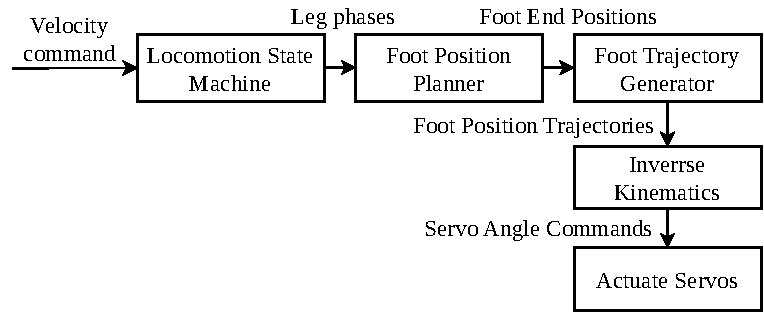
\includegraphics{Diagrams-SysDiffBlockBefore.drawio.pdf}
    \caption{Basic system operation}
    \label{fig:basic_sys}
\end{figure}

\noindent
The basic system will work well enough for walking over flat terrain, but will struggle once any
deviation in terrain height is present. Thus the proposed, more advanced system, operates with the flow shown in figure \ref{fig:adv_sys}.
\begin{figure}[h]
    \centering
    % \hspace{-1.38cm}
    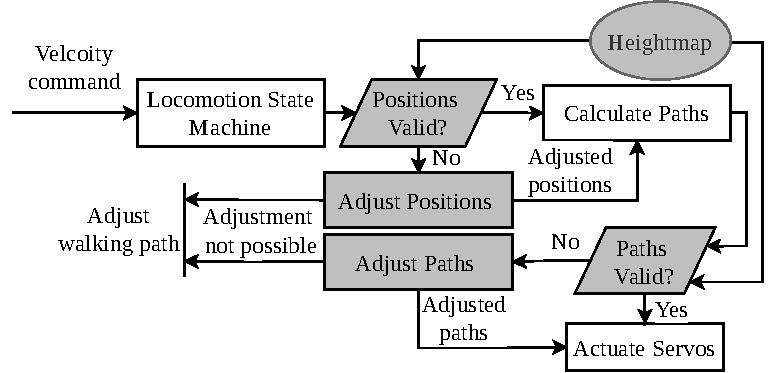
\includegraphics{Diagrams-SysDiffBlockAfter.drawio.pdf}
    \caption{Advanced system operation}
    \label{fig:adv_sys}
\end{figure}

\noindent
The advanced system uses similar components from the basic system, with some differences discussed in
later chapters, but additionally incorporates checks against a heightmap and a score map to validate, and if necessary, adjust the nominal foot 
end positions and paths to move the feet to said positions. If the nominal positions are invalid and no valid adjustment can be made the 
robot will have to change its overall path, however this is not discussed in this paper.

The goal of maneuvering rough terrain is achieved by a combination of 4 primary systems, namely, a mapping, 
foot placement optimisation, motion controller and a \ac*{slam} system. A high level overview of the system implementation can be seen
in figure \ref{fig:system_diagram}.
\begin{figure}[h]
    \centering
    % \hspace{-1.38cm}
    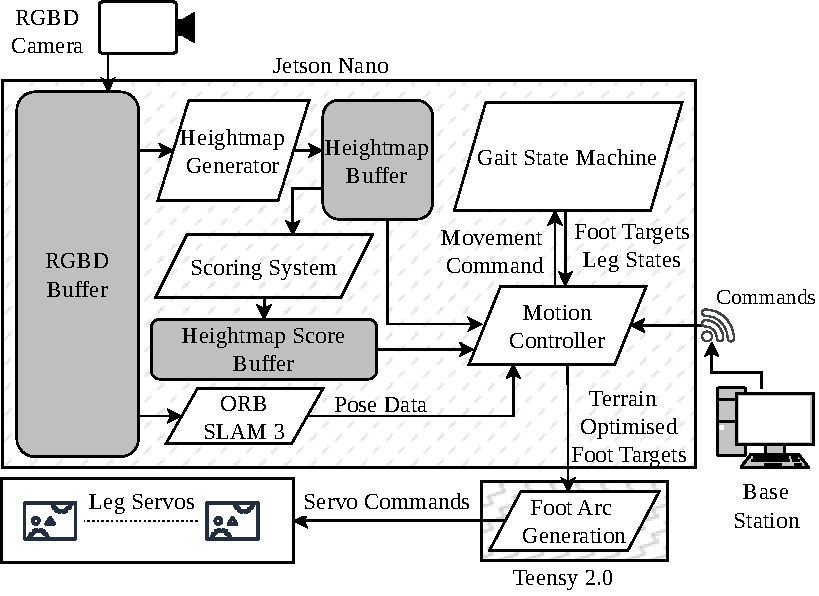
\includegraphics{HexapodSystemDiagram.drawio.pdf}
    \caption{Physical system diagram}
    \label{fig:system_diagram}
\end{figure}

The mapping system utilises the \ac*{rgbd} camera to construct a dense heightmap of the immediate surroundings of the robot, as the robot moves around old data is erased to make
way for new data. The size and resolution of the heightmap is adjustable to the available memory and computational power. The heightmap system is further covered in chapter \ref{chap:mapping}.

The foot placement optimisation system takes the heightmap as input and produces another map of equal size to the heightmap, this new map is the score map and is found by assigning a score to each
cell of the heightmap. The score is dependant on how stable of a place the cell would be for the robot to place its feet. The score map can then be used to evaluate, and adjust if necessary, the
initial foot placement proposed by the motion system. The foot placement optimisation system is further covered in chapter \ref{chap:optimisation}.

All the movement of the robot is handled by the motion system, it is comprised of a gait state machine, a foot target proposal system, a foot arc generator, and \ac{ik}.
The gait state machine selects the swinging and supporting legs during for each step, to achieve a tripod gait. The target proposal system proposes an initial target for all the feet based
on the current step parameters. Simple linear motion is not acceptable for the swinging feet, thus the foot arc generator produces a movement vector based on the remaining distance to a foots destination,
which if followed, results in a arc like motion to the destination. Finally to execute any movements, positions must be converted to angles, and velocity must be converted to
angular rate, thus, and \ac{ik} component is required. The motion system is further covered in chapter \ref{chap:motion}.

\begin{figure}[h]
    \centering
    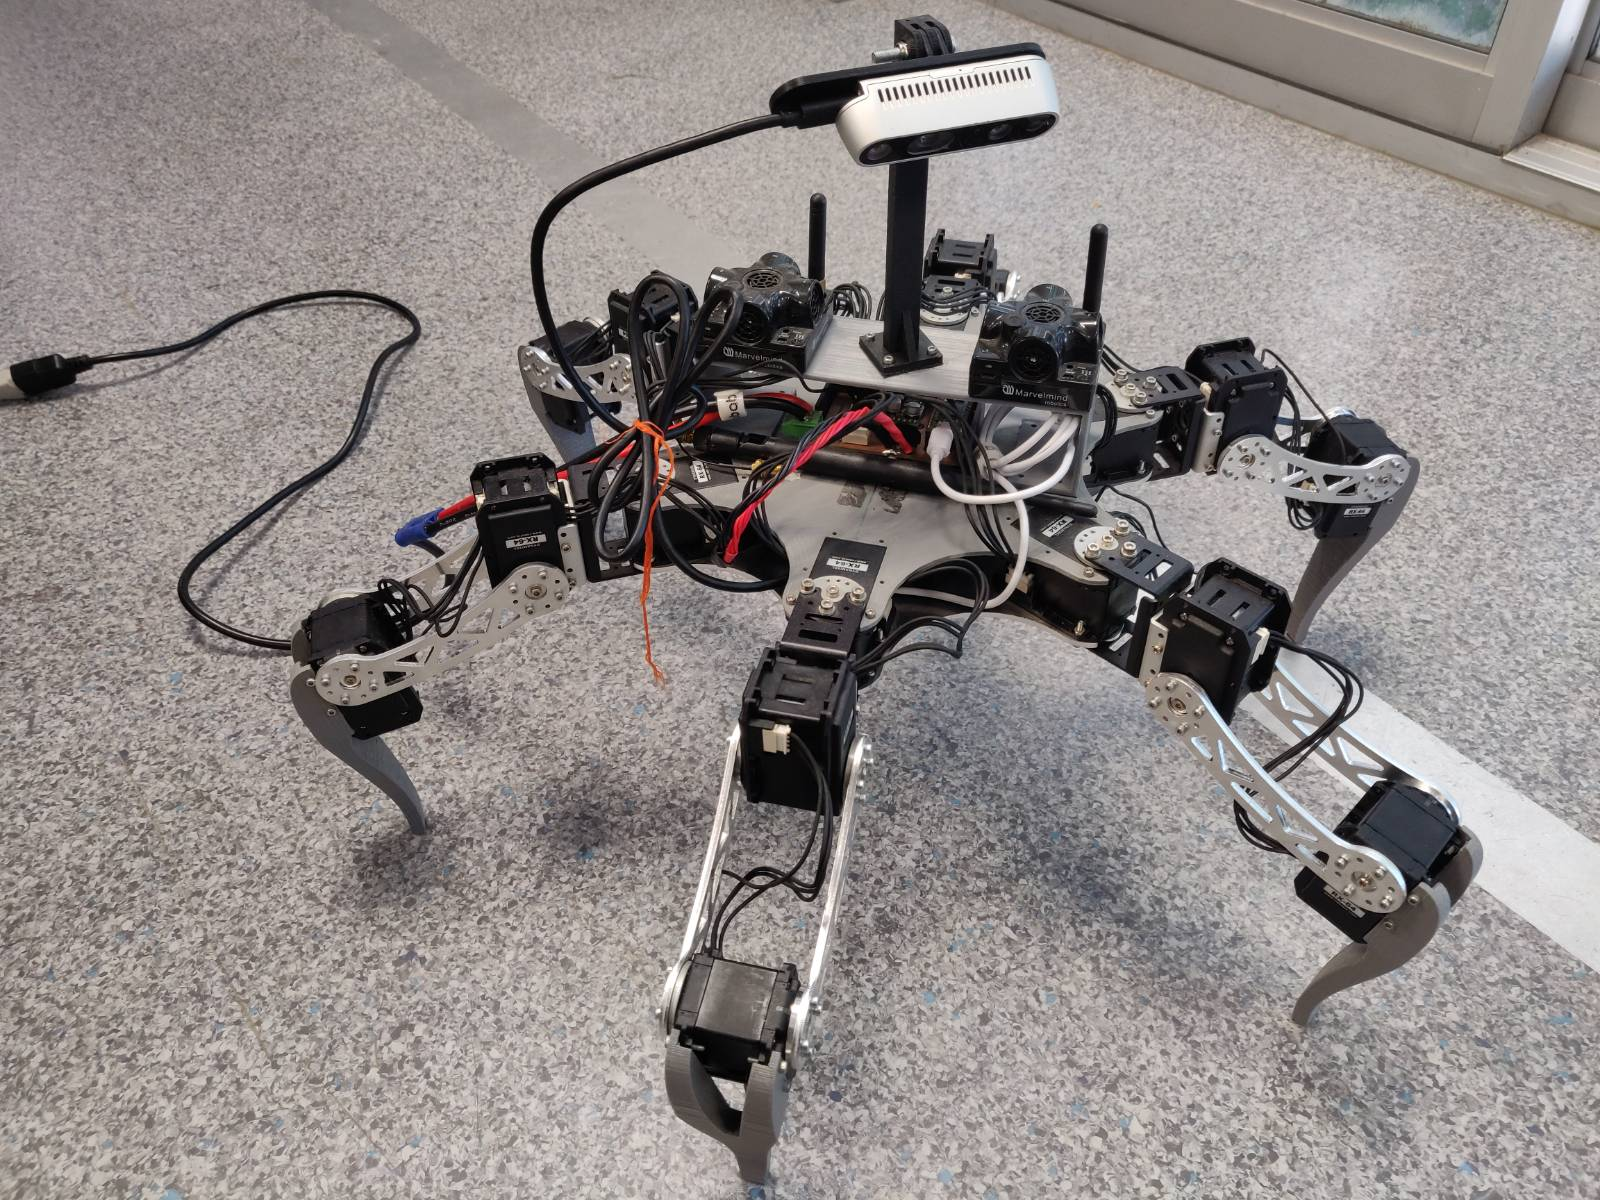
\includegraphics[height=8.5cm]{hexapod.png}
    \caption{Physical Hexapod}
    \label{fig:hexapod}
\end{figure}
